\documentclass[11pt]{article}

\usepackage{sectsty}
\usepackage{graphicx}
\usepackage{hyperref}
\usepackage[style=numeric,backend=biber]{biblatex}

\addbibresource{report.bib}

% Hyperref
\hypersetup{
    colorlinks=true,
    linkcolor=blue,
    filecolor=magenta,
    urlcolor=cyan,
    citecolor=black,
    pdftitle={AR project report},
    pdfpagemode=FullScreen,
}

% Margins
\topmargin=-0.45in
\evensidemargin=0in
\oddsidemargin=0in
\textwidth=6.5in
\textheight=9.0in
\headsep=0.25in

\title{Automated reasoning project report}
\author{Roberto Tonino}
\date{\today}

\begin{document}
\maketitle


\section{Problem statement}

Delle astronavi aliene sono disposte in modo complanare in modo che possiamo immaginarle nel rettangolo cartesiano (0,0), ($max_x$,0), ($max_x$,$max_y$), (0,$max_y$).
$max_x$ e $max_y$ sono dati di input e vengono anche date le coordinate (intere) delle astronavi presenti. Supponiamo non siano già ad ordinata 0 (ovvero sulla terra).

Ci accorgiamo che ad ogni istante di tempo ogni astronave scende unitariamente (ciascuna componente $y$ cala di 1).

Gli alieni sono ostili e vogliamo fermarli.
Disponiamo di un cannone all'inizio in posizione (0,0) che in un istante di tempo può (1) sparare verticalmente distruggendo la astronave più vicina che si trovi nella stessa ascissa, oppure (2) spostarsi (senza sparare) in un'altra ascissa.
Il tempo per spostarsi di 1,2,3,4, etc caselle sull'asse $x$ è sempre unitario.

Si vuole trovare un piano (se esiste) per evitare che anche solo una astronave tocchi terra.

P.S. \'E possibile ci sia una soluzione furba, ad-hoc, per il problema.
Non cerchiamo quella.
Vogliamo codificarlo e fare risolvere al CP solver o al ASP solver.

\section{Clingo model}

In the first few lines we find the domain predicates.
There are a couple of things to note.
The time/1 predicate started from 0.
This is to indiccate the initial state of the world and means that the model will have t+1 time steps.
The x and y axis also start from 0.
This is because the grid is a cartesian rectangle.
The cannon predicate is arguably the most odd: its' written such that the model can have more than one cannon, but practically the model never takes into account this eventuality.
The cannon predicate comes in this shape in order to be able to use a variable C in further predicates.

The alien/1 predicate comes with an identifier, which is simply an integer counter strarting from 1.

The \texttt{1 { ...  } 1} line is a core part of the model.
it states that for each time step except for the last one the cannon either moes to an X or shots an alien.
The last time step is left our because of how the shoot predicate/action is defined further on: when the cannon shoots, an aliens is considered dead in the next time step.

The ``initial state'' predicate uses the at/4 predicate by positioning the cannon at the coordinates 0,0 as required in the problem statement.

The at/4 predicate is also a core part of the model.
At any fiven time step, it represents the position on the grid of the cannon or of an alien.

The model contains the move, shoot actions.
The move/3 action represents only the movement of the cannon.
The requirement of each alien decreasing its y coordinate at every time step is met via an inertia rule.

The shoot/3 action involves both the cannon and an alien.
The cannon shoots an alien A if at time T their x coordinates are equal.

Additionally, we are enforcing the fact that if the cannon shoots, it will stay in the same position in the next time step

The inertia rules involve aliens.
If, at a ceratin point, an alien is dead it will remain dead and it will preserve its position on the grid.
If an alien is not dead, its y coordinate will decrease at each time step.

The constraints avoid the model to accept a solution where the cannon has a y coordinate different than zero---at each time step.
They also avoid a solution where an alien reaches y=0, which would violate the requirements in the problem statement.


\section{Minizinc model}

In the Minizinc model, we define upfront the variables we need the model to assign values to.
The model represents time steps as array indices.
Like in the clingo model, the move\_x and the shoot variables span in t time steps, compared to t+1 timesteps of the other decision variables.

The plannin concepts of precondition and effect are represented by a conjunction.

The concept of action is represented by a quantified boolean formula (QBF): <formula> with A being the set of aliens and T being 0..t timesteps.
The actions are encoded as constraint in the model.

In the model we also find a constraint that enforces, foreach time setep, the move\_x or the shoot actions to not be in their null state.

Inertia rules are represented by a QBF of the form: <formula>.
The idea is to have a if-else-like structure of an imperative programming language.

Finally, the only constraint in the model prohibits the cannon to shoot to teh same alien twice.
This can probably be removed by adding a precondition to the shoot action.


\section{Benchmarks}

\subsection{Instance generation}
Both clingo and minizinc benchmarks were run on 10 instances of aliens.
The instances were generated with the program \texttt{generate.ts} (included in the zip file) that is run with the command

\begin{verbatim}
bun generate.ts <x> <y> <numberOfAliens>
\end{verbatim}

It uses \href{https://bun.sh/}{bun}, a modern TypeScript runtime, but can be ran with node.js as well with some additional work.
The program contains 3 inputs: \texttt{x}, \texttt{y} and \texttt{numberOfAliens}.

The $y$ coordinates of the aliens are generated by taking the input \texttt{y} and decreasing it for each alien present in the instance, obtaining a sequence that starts at $y - 1$ and ends at $y - numberOfAliens$.
The $x$ coordinates of the aliens are randomly generated between 0 and the input \texttt{x}.
This method of generating the coordinates ensures that no aliens are in the same position on the grid.

It is worth noting that if the input \texttt{y} is smaller than $2*numberOfAliens$, the model will most likely be unsatisfiable because the cannon won't be able to kill all the aliens before they reach the $0$ coordinate.
The combination of shoot and move takes 2 time steps.
So, if there are 50 aliens all with different x, 100 time steps are required for the cannon to kill all the aliens before they reach 0.
To enable that, the aliens need to be in a high-enough $y$ coordinate to not reach 0.

\subsection{Minizinc instances}

The \texttt{generate.ts} file generates instances suitable to be used with clingo.
A combination of a shell script, a TypeScript script and a manual step are used to convert them to Minizinc instances.
The two scripts can be found in the zip file and are named \texttt{minizinc/convert} and \texttt{minizinc/convert.ts} respectively.
The \texttt{convert} script creates 10 files names \texttt{aliens.1.mzn}, \texttt{aliens2.mzn}, etc.
The files contain two arrays which values are extracted from \texttt{clingo/aliens1.lp}, \texttt{clingo/aliens2.lp}, etc.
The manual step consists in adding four integer parameters to the files.
The four integer parameters are: \texttt{t}, \texttt{mx} ($max_x$), \texttt{my} ($max_y$), and \texttt{a} (number of aliens).

\subsection{Benchmark setup}

Every instance is ran 10 times with 3 warmup runs.
The clingo model was ran with three different configurations: \textit{auto}, \textit{jumpy}, and \textit{trendy}.
The Minizinc model was ran with two different solvers: default, and \textit{chuffed}.

The results---in JSON format---are stored in the \texttt{clingo/benchmarks} and \texttt{minizinc/benchmarks}.

\subsection{Clingo model}

In \autoref{fig:clingo-bench-comparative} a visualization of the results is presented.
On the x axis there are the 10 aliens files, while on the y axis the runtime of the benchmarks.
There are 3 bars for each file representing the 3 different configurations.
In \autoref{table:clingo-bench-comparative} the full benchmark results is presented.

The \textit{trendy} configuration is the fastest for this problem.
The performance measured on \texttt{aliens8} suggests that \textit{trendy} could be faster when using instances of bigger size.

It is interesting to note how \texttt{aliens3} reaches the timeout with the default configuration, while with \textit{jumpy} and \textit{trendy} the resolution takes around 1 second.
Here's the breakdown of what the configurations are setting (generated by running \texttt{clingo --help=3}):

\begin{verbatim}
[trendy]:
 --sat-p=2,iter=20,occ=25,time=240 --trans-ext=dynamic --heuristic=Vsids
 --restarts=D,100,0.7 --deletion=basic,50 --del-init=3.0,500,19500
 --del-grow=1.1,20.0,x,100,1.5 --del-cfl=+,10000,2000 --del-glue=2
 --strengthen=recursive --update-lbd=less --otfs=2 --save-p=75
 --counter-restarts=3,1023 --reverse-arcs=2 --contraction=250 --loops=common
[jumpy]:
 --sat-p=2,iter=20,occ=25,time=240 --trans-ext=dynamic --heuristic=Vsids
 --restarts=L,100 --deletion=basic,75,mixed --del-init=3.0,1000,20000
 --del-grow=1.1,25,x,100,1.5 --del-cfl=x,10000,1.1 --del-glue=2
 --update-lbd=glucose --strengthen=recursive --otfs=2 --save-p=70
\end{verbatim}

From these exaustive lists of command line flags, we can extract simply \texttt{--sat-p=2} to get a significative performance improvement.
The flag enables ``SAT preprocessing'', more precisely ``SatELite-like'' preprocessing \cite{clingo-guide}.
SAT preprocessing alone shows a 13-fold improvement, as presented in \autoref{table:aliens3-sat-p}.

\begin{table}
  \centering
  \begin{tabular}{|llrrrrrr|}
    \hline
    Aliens & Configuration & Mean & Std Dev & Min & Max & Times faster & Percentage \\
    \hline
    aliens3 & auto & 300.01~s & 0.0012~s & 300.00~s & 300.01~s & 1.0x & baseline \\
    aliens3 & \texttt{--sat-p=2} & 23.06~s & 0.99~s & 21.59~s & 24.67~s & 13.0x & -92.31\% \\
    \hline
  \end{tabular}
  \caption{\texttt{aliens3} with \texttt{sat-p} flag}
  \label{table:aliens3-sat-p}
\end{table}

When the search space becomes of considerable dimensions, the \textit{auto} configuration struggles.
It almost reaches the timeout with \texttt{alien6} and always reaches it from \texttt{aliens7} upwards.
\textit{Jumpy} and \textit{trendy} perform well under the timeout with \texttt{aliens6}, but reach it with \texttt{aliens7}.
With \texttt{aliens8} both configurations run well under the timeout, with \textit{trendy} running under the minute threshold.

\begin{figure}[h]
  \centering
  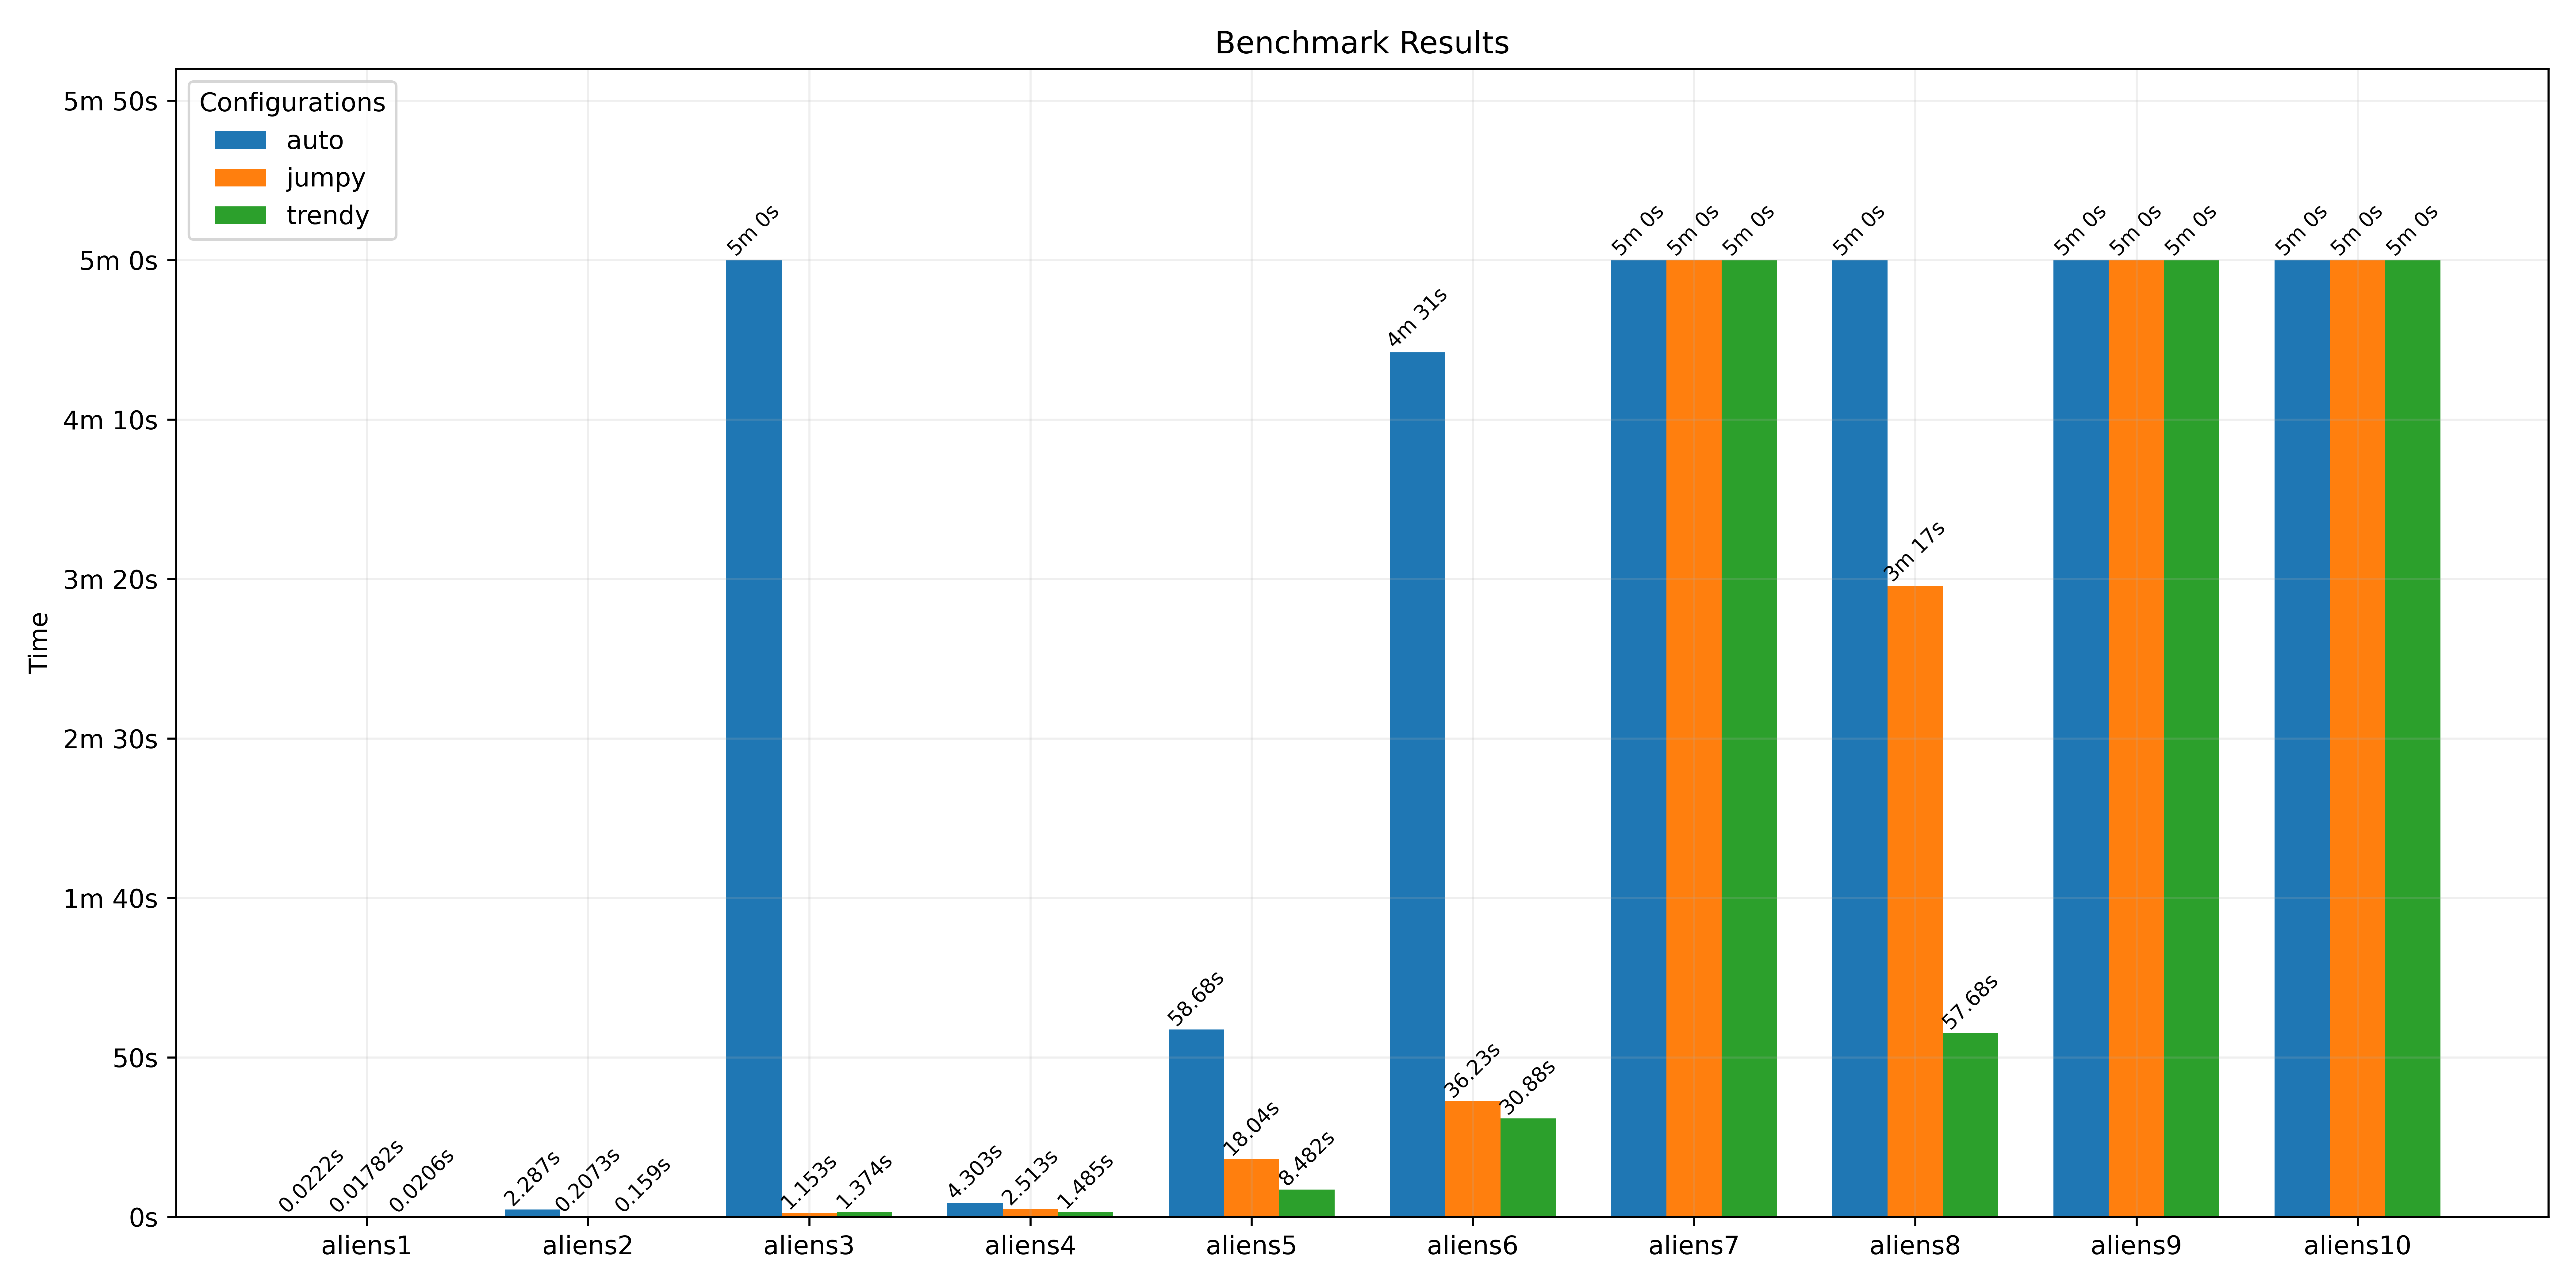
\includegraphics[width=\textwidth]{./clingo/benchmarks/balanced_comparative.png}
  \caption{Comparing clingo benchmark results}
  \label{fig:clingo-bench-comparative}
\end{figure}


% \begin{table}[h]
%   \centering
%   \begin{tabular}{|c|c|c|c|c|}
%     \hline
%     File & Number of aliens & $max_x$ & $max_y$ & $t$ \\
%     \hline
%     aliens1.lp & 3 & 9 & 9 & 5 \\
%     aliens2.lp & 9 & 10 & 21 & 18 \\
%     aliens3.lp & 15 & 15 & 40 & 28 \\
%     aliens4.lp & 20 & 20 & 50 & 42 \\
%     aliens5.lp & 25 & 15 & 75 & 44 \\
%     aliens6.lp & 30 & 50 & 80 & 58 \\
%     aliens7.lp & 35 & 30 & 100 & 67 \\
%     aliens8.lp & 40 & 100 & 100 & 82 \\
%     aliens9.lp & 50 & 20 & 110 & 90 \\
%     aliens10.lp & 100 & 70 & 250 & 202 \\
%     \hline
%   \end{tabular}
%   \caption{Instances used for benchmarking the model}
%   \label{table:clingo-bench-instances}
% \end{table}

\begin{table}[h]
  \centering
  \begin{tabular}{|llrrrrrr|}
    \hline
    Aliens & Configuration & Mean & Std Dev & Min & Max & Times faster & Percentage \\
    \hline
    aliens1 & auto & 0.022~s & 0.008~s & 0.014~s & 0.039~s & 1.0x & baseline \\
    aliens1 & jumpy & 0.018~s & 0.0016~s & 0.015~s & 0.021~s & 1.2x & -19.76\% \\
    aliens1 & trendy & 0.021~s & 0.0016~s & 0.019~s & 0.024~s & 1.1x & -7.21\% \\
    \hline
    aliens2 & auto & 2.29~s & 0.6~s & 1.84~s & 3.48~s & 1.0x & baseline \\
    aliens2 & jumpy & 0.21~s & 0.0093~s & 0.19~s & 0.22~s & 11.0x & -90.93\% \\
    aliens2 & trendy & 0.16~s & 0.015~s & 0.15~s & 0.2~s & 14.4x & -93.05\% \\
    \hline
    aliens3 & auto & 300.01~s & 0.0012~s & 300.00~s & 300.01~s & 1.0x & baseline \\
    aliens3 & jumpy & 1.15~s & 0.044~s & 1.12~s & 1.27~s & 260.2x & -99.62\% \\
    aliens3 & trendy & 1.37~s & 0.017~s & 1.35~s & 1.40~s & 218.3x & -99.54\% \\
    \hline
    aliens4 & auto & 4.30~s & 0.049~s & 4.24~s & 4.39~s & 1.0x & baseline \\
    aliens4 & jumpy & 2.51~s & 0.026~s & 2.48~s & 2.55~s & 1.7x & -41.60\% \\
    aliens4 & trendy & 1.48~s & 0.022~s & 1.45~s & 1.51~s & 2.9x & -65.50\% \\
    \hline
    aliens5 & auto & 58.68~s & 0.38~s & 58.16~s & 59.30~s & 1.0x & baseline \\
    aliens5 & jumpy & 18.04~s & 0.18~s & 17.83~s & 18.46~s & 3.3x & -69.26\% \\
    aliens5 & trendy & 8.48~s & 0.13~s & 8.35~s & 8.80~s & 6.9x & -85.54\% \\
    \hline
    aliens6 & auto & 271.09~s & 0.52~s & 270.06~s & 271.75~s & 1.0x & baseline \\
    aliens6 & jumpy & 36.23~s & 0.34~s & 35.89~s & 36.80~s & 7.5x & -86.63\% \\
    aliens6 & trendy & 30.88~s & 0.45~s & 30.43~s & 31.79~s & 8.8x & -88.61\% \\
    \hline
    aliens7 & auto & 300.01~s & 0.0025~s & 300.00~s & 300.01~s & 1.0x & baseline \\
    aliens7 & jumpy & 300.01~s & 0.00071~s & 300.00~s & 300.01~s & 1.0x & -0.00\% \\
    aliens7 & trendy & 300.01~s & 0.00055~s & 300.00~s & 300.01~s & 1.0x & -0.00\% \\
    \hline
    aliens8 & auto & 300.01~s & 0.0014~s & 300.01~s & 300.01~s & 1.0x & baseline \\
    aliens8 & jumpy & 197.89~s & 1.78~s & 196.43~s & 202.73~s & 1.5x & -34.04\% \\
    aliens8 & trendy & 57.68~s & 0.29~s & 57.30~s & 58.29~s & 5.2x & -80.77\% \\
    \hline
    aliens9 & auto & 300.01~s & 0.0018~s & 300.01~s & 300.01~s & 1.0x & baseline \\
    aliens9 & jumpy & 300.01~s & 0.0064~s & 300.01~s & 300.03~s & 1.0x & +0.00\% \\
    aliens9 & trendy & 300.01~s & 0.0011~s & 300.00~s & 300.01~s & 1.0x & -0.00\% \\
    \hline
    aliens10 & auto & 300.01~s & 0.0016~s & 300.01~s & 300.01~s & 1.0x & baseline \\
    aliens10 & jumpy & 300.01~s & 0.0022~s & 300.01~s & 300.02~s & 1.0x & +0.00\% \\
    aliens10 & trendy & 300.01~s & 0.0011~s & 300.01~s & 300.01~s & 1.0x & -0.00\% \\
    \hline
  \end{tabular}
  \caption{Complete clingo benchmark results}
  \label{table:clingo-bench-comparative}
\end{table}

\subsection{Minizinc model}

The \texttt{org.chuffed.chuffed} solver has a huge benefit in \texttt{aliens2}.
This advantage vanishes starting with \texttt{aliens3}.
From \texttt{aliens3} to \texttt{aliens10} the model, ran with the default solver and with \texttt{org.chuffed.chuffed}, always reaches the timeout.

This means that the model solves the problem, but there's room for improvement.


\begin{figure}[h]
  \centering
  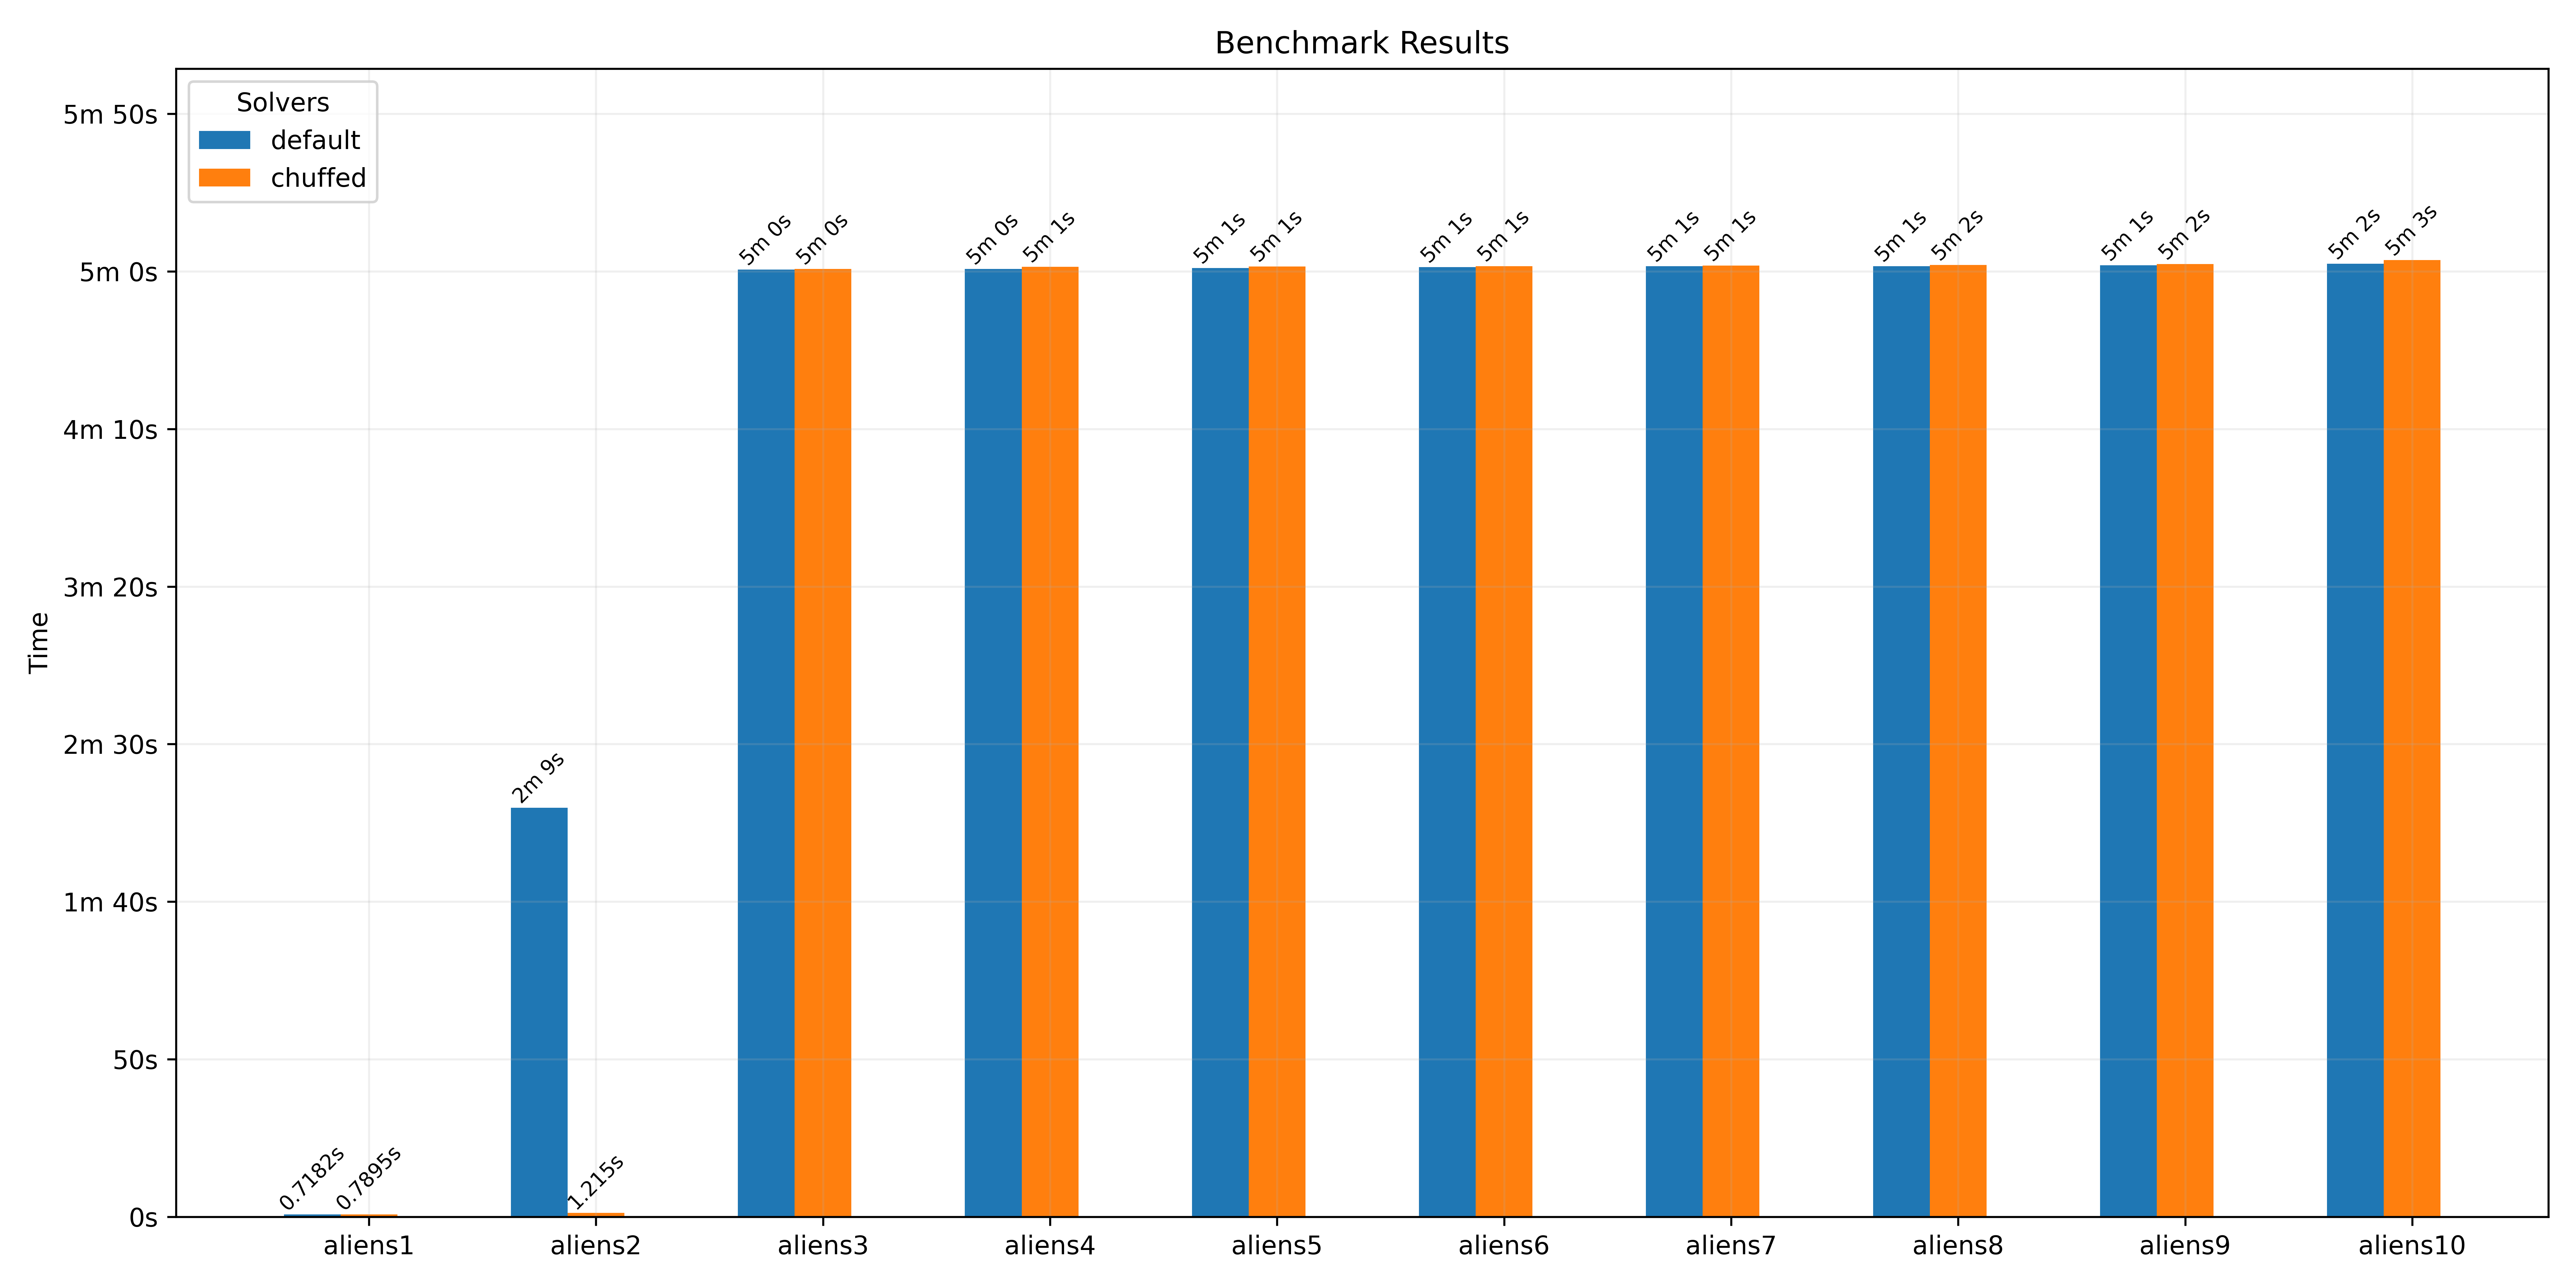
\includegraphics[width=\textwidth]{./minizinc/benchmarks/balanced_comparative.png}
  \caption{Comparing minizinc benchmark results}
  \label{fig:minizinc-bench-comparative}
\end{figure}

\section{Conclusion}
The clingo and the minizinc model are similar in terms of clauses and constraints.
The difference of results between the benchmark runs is due to the default behaviours of the two programs.
As clingo is generally used for ASP solving and Minizinc is used for CSP solving, the scope of the programs is different.

The problem proposed for this project is a \textit{planning} problem, requiring adaptation from the planning domain to the ASP or CSP domain.

\begin{table}[h]
  \centering
  \begin{tabular}{|llrrrrrr|}
    \hline
    Aliens & Solver & Mean & Std Dev & Min & Max & Times faster & Percentage \\
    \hline
    aliens1 & default & 0.72~s & 0.034~s & 0.68~s & 0.8~s & 1.0x & baseline \\
    aliens1 & chuffed & 0.79~s & 0.048~s & 0.74~s & 0.86~s & 0.9x & +9.94\% \\
    \hline
    aliens2 & default & 129.84~s & 3.59~s & 123.64~s & 136.12~s & 1.0x & baseline \\
    aliens2 & chuffed & 1.22~s & 0.041~s & 1.17~s & 1.28~s & 106.8x & -99.06\% \\
    \hline
    aliens3 & default & 300.58~s & 0.027~s & 300.55~s & 300.64~s & 1.0x & baseline \\
    aliens3 & chuffed & 300.77~s & 0.041~s & 300.73~s & 300.86~s & 1.0x & +0.06\% \\
    \hline
    aliens4 & default & 300.80~s & 0.025~s & 300.75~s & 300.84~s & 1.0x & baseline \\
    aliens4 & chuffed & 301.44~s & 0.042~s & 301.40~s & 301.54~s & 1.0x & +0.22\% \\
    \hline
    aliens5 & default & 301.09~s & 0.036~s & 301.02~s & 301.13~s & 1.0x & baseline \\
    aliens5 & chuffed & 301.60~s & 0.024~s & 301.55~s & 301.65~s & 1.0x & +0.17\% \\
    \hline
    aliens6 & default & 301.37~s & 0.02~s & 301.34~s & 301.41~s & 1.0x & baseline \\
    aliens6 & chuffed & 301.70~s & 0.027~s & 301.65~s & 301.74~s & 1.0x & +0.11\% \\
    \hline
    aliens7 & default & 301.66~s & 0.038~s & 301.60~s & 301.72~s & 1.0x & baseline \\
    aliens7 & chuffed & 301.86~s & 0.031~s & 301.81~s & 301.91~s & 1.0x & +0.07\% \\
    \hline
    aliens8 & default & 301.62~s & 0.065~s & 301.57~s & 301.79~s & 1.0x & baseline \\
    aliens8 & chuffed & 302.06~s & 0.044~s & 302.01~s & 302.15~s & 1.0x & +0.15\% \\
    \hline
    aliens9 & default & 301.97~s & 0.063~s & 301.89~s & 302.08~s & 1.0x & baseline \\
    aliens9 & chuffed & 302.31~s & 0.032~s & 302.27~s & 302.38~s & 1.0x & +0.11\% \\
    \hline
    aliens10 & default & 302.41~s & 0.065~s & 302.33~s & 302.57~s & 1.0x & baseline \\
    aliens10 & chuffed & 303.61~s & 0.89~s & 302.86~s & 305.96~s & 1.0x & +0.40\% \\

    \hline
  \end{tabular}
  \caption{Complete minizinc benchmark results}
  \label{table:minizinc-bench-comparative}
\end{table}

\section{Future work}
Several implementations can be done to speed up the solving of the models.
Both the clingo and Minizinc models do not have constraints on how the cannon should move or shoot.
The cannon can be constrained to move to the closest alien or to shoot to all the aliens in the same $x$ coordinate as where the cannon is at a specific time step.


\printbibliography

\end{document}
